\documentclass[tikz,border=10pt]{standalone}
\usepackage{amsmath}
\usepackage{tikz}
\usetikzlibrary{arrows.meta, positioning, calc, shapes.geometric, fit, backgrounds}

\begin{document}
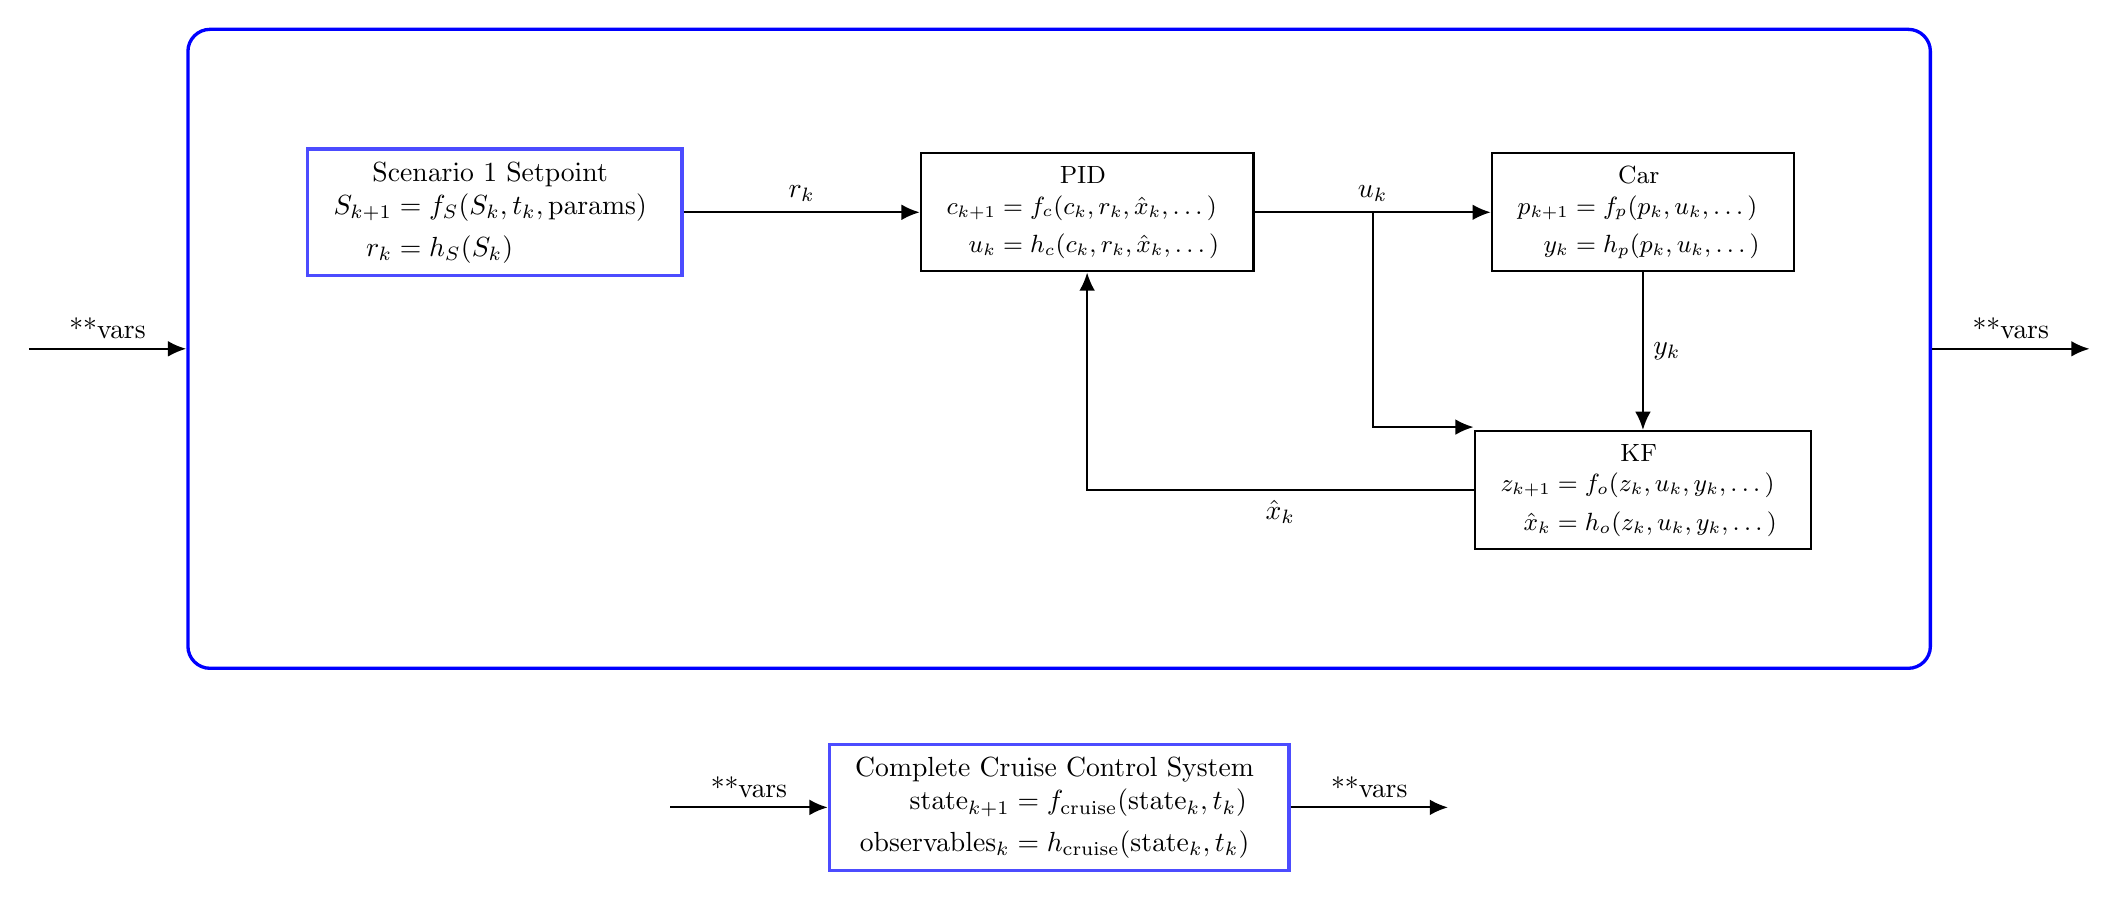
\begin{tikzpicture}[
  block/.style = {
    draw,
    thick,
    minimum height=2.5em,
    minimum width=5em,
    align=center,
    font=\small
  },
  wrapper/.style = {
    draw=blue,
    very thick,
    rounded corners=8pt,
    inner sep=1.5cm
  },
  blueblock/.style = {
    draw=blue!70,
    very thick,
    minimum height=3em,
    minimum width=8em,
    align=center
  },
  arrow/.style = {thick, -{Latex[width=2mm]}},
  node distance=1.8cm and 1.8cm
]

% ======================================================
% TOP SYSTEM
% ======================================================

\node[blueblock] (setpoint) {
  \begin{tabular}{c}
    Scenario 1 Setpoint \\
    $\begin{aligned}
      S_{k+1} &= f_S(S_k, t_k, \mathrm{params}) \\
      r_k &= h_S(S_k)
    \end{aligned}$
  \end{tabular}
};

\node[block, right=3cm of setpoint] (controller) {
  \begin{tabular}{c}
    PID\\
    $\begin{aligned}
      c_{k+1} &= f_c(c_k, r_k, \hat{x}_k, \dots) \\
      u_k &= h_c(c_k, r_k, \hat{x}_k, \dots)
    \end{aligned}$
  \end{tabular}
};

\node[block, right=3cm of controller] (system) {
  \begin{tabular}{c}
    Car\\
    $\begin{aligned}
      p_{k+1} &= f_p(p_k, u_k, \dots) \\
      y_k &= h_p(p_k, u_k, \dots)
    \end{aligned}$
  \end{tabular}
};

\node[block, below=2cm of system] (observer) {
  \begin{tabular}{c}
    KF\\
    $\begin{aligned}
      z_{k+1} &= f_o(z_k, u_k, y_k, \dots) \\
      \hat{x}_k &= h_o(z_k, u_k, y_k, \dots)
    \end{aligned}$
  \end{tabular}
};

% ---- Arrows ----
\draw[arrow] (setpoint.east) -- node[above] {$r_k$} (controller.west);
\draw[arrow] (controller.east) -- node[above] {$u_k$} (system.west);
\draw[arrow] (system.south) -- node[right] {$y_k$} (observer.north);

% u_k split to observer
\coordinate (usplit) at ($(controller.east)!0.5!(system.west)$);
\draw[arrow] (usplit) |- ($(observer.west)+(0,0.8)$);

% xhat feedback
\draw[arrow] (observer.west) -| node[pos=0.25, below] {$\hat{x}_k$} (controller.south);

% ---- Wrapper ----
\begin{scope}[on background layer]
  \node[wrapper, fit=(setpoint)(controller)(system)(observer)] (wrap_top) {};
\end{scope}

% External arrows
\draw[arrow] ($(wrap_top.west)+(-2,0)$) -- node[above] {**vars} (wrap_top.west);
\draw[arrow] (wrap_top.east) -- ++(2,0) node[midway, above] {**vars};

% ======================================================
% BOTTOM SYSTEM
% ======================================================

\node[blueblock, below=5cm of wrap_top.center] (cruise) {
  \begin{tabular}{c}
    Complete Cruise Control System\\
    $\begin{aligned}
      \mathrm{state}_{k+1} &= f_{\mathrm{cruise}}(\mathrm{state}_k, t_k) \\
      \mathrm{observables}_k &= h_{\mathrm{cruise}}(\mathrm{state}_k, t_k)
    \end{aligned}$
  \end{tabular}
};

\draw[arrow] ($(cruise.west)+(-2,0)$) -- node[above] {**vars} (cruise.west);
\draw[arrow] (cruise.east) -- ++(2,0) node[midway, above] {**vars};

\end{tikzpicture}
\end{document}
